% Drawing 154/06-6 -- folder 154, batch 06, archive page 109 (PDF page 110).
% Transcription: dessins en couleur sans texte : des droites vert clair orientées (flèche vers la gauche) coupées de droites rouges, verticales ou croisées deux à deux ; les droites vertes montent en marche d'escalier ou contournent les croisements, et des arcs sont renforcés en noir ; de fines flèches au crayon, numérotées $1$, $2$, $3$, indiquent les déplacements successifs. En bas à gauche, un croisement de deux droites rouges sur deux droites (vert clair et vert foncé), avec un petit cercle fléché autour du point
% Kind: oriented lines cut by red lines, climbing in steps or going round crossings. Method 2 (schematic redraw from the facsimile). Status: partial.
% Notes: Colour drawings without text, on a printed listing (upside-down job log, not reproduced): light green oriented lines (arrow to the left) cut by red lines, vertical or crossed in pairs; the green lines climb in steps or go round the crossings, and arcs are reinforced in black; fine pencil arrows numbered 1, 2, 3 for the successive moves (left out). Bottom left, a crossing of two red lines on two lines (light green and dark green), with a small arrowed circle round the point. The pencil sketches at the lower right and the red line at the top are not reproduced in detail (the red line is drawn). Read from the page view. Still differs from the facsimile: Colour drawings without text, on a printed listing (upside-down job log, not reproduced): light green oriented lines (arrow to the left) cut by red lines, vertical or crossed in pairs; the green lines climb in steps or go round the crossings, and arcs are reinforced in black; fine pencil arrows numbered 1, 2, 3 for the successive moves (left out). The pencil sketches at the lower right and the red line at the top are not reproduced in detail (the red line is drawn).
% Coordinates: 1 unit = 1 mm = 1/100 of the crop width (bbox in page fractions: [0.152, 0.146, 0.9, 0.509]).
% Redrawn by Claude (claude-opus-5-5), issue #73, 2026-11-07; not checked by a human; not compiled (no TeX in the session).
% Revised by Claude (claude-opus-5-5) 2026-11-09 (issue #128) after Michel's check: vertices snapped to exact intersections (drawn points on their lines, meeting ends on the stroke they meet, near-concurrent lines through one computed point, curve ends on their rim); labels at \small as in folder 80 batch 3. Status: partial.
% Rights: reproduces part of the work -- behind RENDER_TRANSCRIPTS, never published by itself.
\documentclass[tikz,border=3pt]{standalone}
\usepackage{amsmath,amssymb}
\usetikzlibrary{patterns,arrows.meta}
\tikzset{Or/.style={orange!90!black}, Ye/.style={yellow!80!orange}, Lg/.style={green!60!black!70}, Dg/.style={green!45!black}, Br/.style={brown!80!black}, Rd/.style={red!85!black}, Bl/.style={blue!70!black}, Gy/.style={black!40}, pencil/.style={black!45}, struck/.style={black!35}, mark/.style={circle,draw,inner sep=1.3pt}, pt/.style={circle,fill,inner sep=0.9pt}, opt/.style={circle,draw,fill=white,inner sep=1.1pt}}
\begin{document}
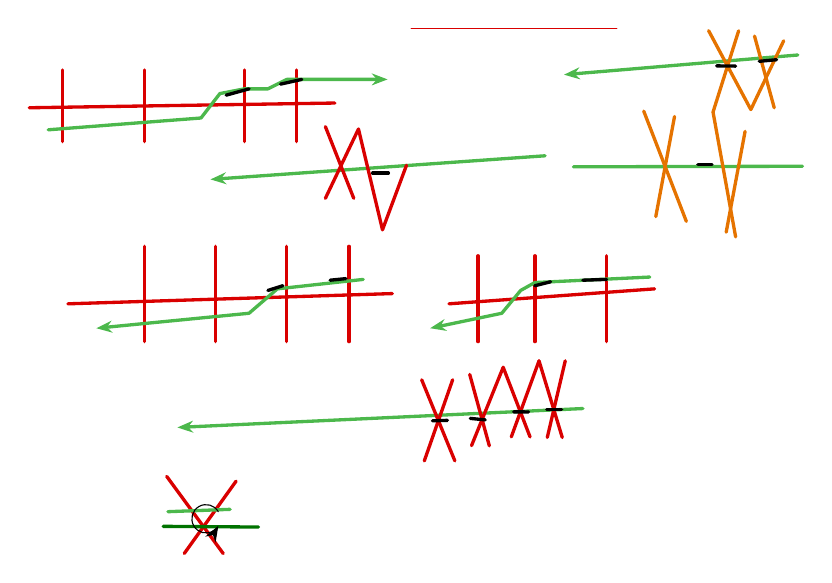
\begin{tikzpicture}[x=1mm,y=1mm,line cap=round,line join=round,font=\scriptsize]
\draw[Rd] (49.1,-0.8) -- (75.2,-0.8);
\draw[Rd,very thick] (0.6,-10.9) -- (39.4,-10.3);
\draw[Rd,very thick] (4.8,-6.1) -- (4.8,-15.2);
\draw[Rd,very thick] (15.2,-6.1) -- (15.2,-15.2);
\draw[Rd,very thick] (27.9,-6.1) -- (27.9,-15.2);
\draw[Rd,very thick] (34.5,-6.1) -- (34.5,-15.2);
\draw[Lg,very thick,-{Stealth[length=2mm]}] (3,-13.7) -- (22.4,-12.2) -- (24.8,-9.1) -- (27.9,-8.5) -- (30.9,-8.5) -- (33.3,-7.3) -- (46.1,-7.3);
\draw[very thick] (25.6,-9.3) -- (28.5,-8.5);
\draw[very thick] (32.5,-7.9) -- (35.2,-7.3);
\draw[Lg,very thick,-{Stealth[length=2mm]}] (66.1,-17) -- (23.6,-20);
\draw[Rd,very thick] (38.2,-13.3) -- (41.8,-22.4);
\draw[Rd,very thick] (42.4,-13.6) -- (38.2,-22.4);
\draw[Rd,very thick] (42.4,-13.6) -- (45.45,-26.4);
\draw[Rd,very thick] (48.5,-18.2) -- (45.45,-26.4);
\draw[very thick] (44.2,-19.2) -- (46.2,-19.2);
\draw[Lg,very thick,-{Stealth[length=2mm]}] (98.2,-4.2) -- (68.5,-6.7);
\draw[Or,very thick] (86.87,-1.11) -- (92.23,-11.13);
\draw[Or,very thick] (90.68,-1.13) -- (87.43,-11.45);
\draw[Or,very thick] (92.7,-1.8) -- (95.2,-10.9);
\draw[Or,very thick] (96.4,-2.4) -- (92.23,-11.13);
\draw[very thick] (87.9,-5.58) -- (90.3,-5.61);
\draw[very thick] (93.3,-5) -- (95.5,-4.8);
\draw[Lg,very thick] (69.7,-18.4) -- (98.8,-18.33);
\draw[Or,very thick] (78.63,-11.33) -- (84.04,-25.33);
\draw[Or,very thick] (82.54,-12.01) -- (80.16,-24.72);
\draw[Or,very thick] (87.43,-11.45) -- (90.3,-27.3);
\draw[Or,very thick] (91.5,-13.9) -- (89.1,-26.7);
\draw[very thick] (85.5,-18.1) -- (87.3,-18.1);
\draw[Rd,very thick] (5.5,-35.8) -- (46.7,-34.5);
\draw[Rd,very thick] (15.2,-28.5) -- (15.2,-40.6);
\draw[Rd,very thick] (24.2,-28.5) -- (24.2,-40.6);
\draw[Rd,very thick] (33.3,-28.5) -- (33.3,-40.6);
\draw[Rd,very thick] (41.2,-28.5) -- (41.2,-40.6);
\draw[Lg,very thick,-{Stealth[length=2mm]}] (43,-32.7) -- (32.1,-33.9) -- (28.5,-37) -- (9.1,-38.9);
\draw[very thick] (30.9,-34.1) -- (32.8,-33.5);
\draw[very thick] (38.8,-32.8) -- (40.8,-32.6);
\draw[Rd,very thick] (53.9,-35.8) -- (80,-33.9);
\draw[Rd,very thick] (57.6,-29.7) -- (57.6,-40.6);
\draw[Rd,very thick] (64.8,-29.7) -- (64.8,-40.6);
\draw[Rd,very thick] (73.9,-29.7) -- (73.9,-40.6);
\draw[Lg,very thick,-{Stealth[length=2mm]}] (79.4,-32.4) -- (64.8,-33.1) -- (63,-34.1) -- (60.6,-37) -- (51.5,-38.9);
\draw[very thick] (64.8,-33.5) -- (66.8,-33);
\draw[very thick] (70.9,-32.8) -- (73.9,-32.7);
\draw[Lg,very thick,-{Stealth[length=2mm]}] (70.9,-49.1) -- (19.4,-51.5);
\draw[Rd,very thick] (50.43,-45.45) -- (54.64,-55.74);
\draw[Rd,very thick] (54.36,-45.45) -- (50.76,-55.75);
\draw[Rd,very thick] (56.53,-44.77) -- (59.02,-53.84);
\draw[Rd,very thick] (60.78,-43.86) -- (56.76,-53.81);
\draw[Rd,very thick] (60.78,-43.86) -- (64.19,-52.7);
\draw[Rd,very thick] (65.33,-43.04) -- (61.81,-52.7);
\draw[Rd,very thick] (65.33,-43.04) -- (68.28,-52.77);
\draw[Rd,very thick] (68.66,-43.04) -- (66.38,-52.77);
\draw[very thick] (51.8,-50.66) -- (53.7,-50.6);
\draw[very thick] (56.6,-50.35) -- (58.49,-50.54);
\draw[very thick] (62.1,-49.52) -- (64,-49.53);
\draw[very thick] (66.3,-49.23) -- (68.2,-49.23);
\draw[Rd,very thick] (18.05,-57.72) -- (25.22,-67.51);
\draw[Rd,very thick] (26.86,-58.32) -- (20.28,-67.5);
\draw[Lg,very thick] (18.2,-62.2) -- (26.1,-61.9);
\draw[Dg,very thick] (17.6,-64.06) -- (29.7,-64.15);
\draw[-{Stealth[length=2mm]}] (24.6,-62.2) arc[start angle=30, end angle=330, x radius=1.8, y radius=1.8];
\end{tikzpicture}
\end{document}
